%%%%%%%%%%%%%%%%%%%%%%%%%%%%%%%%%%%%%%%%%%%%%%%%%%%%%%%%%%%%%%%%%%%%%%%%%%%%%%%%%%%%%%%%%%%%%%%%%%%%%%%%%%%%%%%%%%%%%%%%%%%%%%%%%%%%%%%%%%%%%%%%%%%%%%%%%%%%%%%%%%%
% Written By Michael Brodskiy
% Class: Fundamentals of Electronics
% Professor: M. Onabajo
%%%%%%%%%%%%%%%%%%%%%%%%%%%%%%%%%%%%%%%%%%%%%%%%%%%%%%%%%%%%%%%%%%%%%%%%%%%%%%%%%%%%%%%%%%%%%%%%%%%%%%%%%%%%%%%%%%%%%%%%%%%%%%%%%%%%%%%%%%%%%%%%%%%%%%%%%%%%%%%%%%%

\documentclass[12pt]{article} 
\usepackage{alphalph}
\usepackage[utf8]{inputenc}
\usepackage[russian,english]{babel}
\usepackage{titling}
\usepackage{amsmath}
\usepackage{graphicx}
\usepackage{enumitem}
\usepackage{amssymb}
\usepackage[super]{nth}
\usepackage{everysel}
\usepackage{ragged2e}
\usepackage{geometry}
\usepackage{multicol}
\usepackage{fancyhdr}
\usepackage{cancel}
\usepackage{siunitx}
\usepackage{physics}
\usepackage{tikz}
\usepackage{mathdots}
\usepackage{yhmath}
\usepackage{cancel}
\usepackage{color}
\usepackage{array}
\usepackage{multirow}
\usepackage{gensymb}
\usepackage{tabularx}
\usepackage{extarrows}
\usepackage{booktabs}
\usepackage{lastpage}
\usetikzlibrary{fadings}
\usetikzlibrary{patterns}
\usetikzlibrary{shadows.blur}
\usetikzlibrary{shapes}

\geometry{top=1.0in,bottom=1.0in,left=1.0in,right=1.0in}
\newcommand{\subtitle}[1]{%
  \posttitle{%
    \par\end{center}
    \begin{center}\large#1\end{center}
    \vskip0.5em}%

}
\usepackage{hyperref}
\hypersetup{
colorlinks=true,
linkcolor=blue,
filecolor=magenta,      
urlcolor=blue,
citecolor=blue,
}


\title{Lecture 2}
\date{\today}
\author{Michael Brodskiy\\ \small Professor: M. Onabajo}

\begin{document}

\maketitle

\begin{itemize}

  \item Current-Amplifier Model

    \begin{figure}[H]
      \centering
      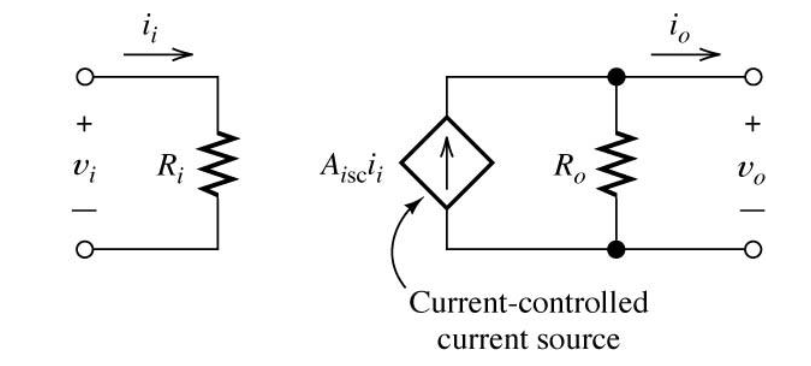
\includegraphics[width=.7\textwidth]{Images/CAM.png}
      \caption{Reference Figure for Current-Amplifier Model}
      \label{fig:1}
    \end{figure}

    \begin{itemize}

      \item Parameters

        \begin{itemize}

          \item $i_i$ is the input current, which ideally comes from a current source

          \item $R_i$ and $R_o$ are the input and output resistances, respectively

          \item $A_{isc}$ is the short-circuit current gain

        \end{itemize}

      \item Current gain with load impedance at the output: $A_i=i_o/i_i$

    \end{itemize}

  \item Application of Th\'evenin to Norton transformation

    \begin{itemize}

      \item The connection of $R_o$ is changed, but the value remains the same

    \end{itemize}

  \item $A_{isc}=i_{osc}/i_i$ is obtained with a short-circuit at the output terminals

    \begin{itemize}

      \item where: $i_{osc}=A_{vo}v_i/R_o$ and $i_i=v_i/R_i$

      \item After substituting: $A_{isc}=A_{vo}(R_i/R_o)$

    \end{itemize}

\end{itemize}

\end{document}

